\chapter{Criticality Safety}
\label{lec:criticalitysafety}

In this lecture, we discuss the topic of \textit{criticality safety}, one 
of the most important physics-oriented aspects of nuclear engineering not 
specifically dealing with core physics, beginning with a brief  
overview.  Thereafter, the chief physical concerns related to criticality 
safety are described and illustrated with a simple example, and a few 
notable 
accidents over the past several decades are described.  Finally, 
computational aspects of criticality safety are discussed, and the topic 
of burnup credit is used as a case study to illustrate recent efforts in 
criticality safety analysis.

%------------------------------------------------------------------------------
% OVERVIEW
%------------------------------------------------------------------------------

\section*{Overview}

\textit{Nuclear criticality safety}, 
as defined by the American National Standard ANSI/ANS 8.1 \cite{ans8.1}, is 
the ``protection against the consequences of a criticality safety
accident, preferably by prevention of the accident,'' and it defines
a \textit{criticality accident} as ``the release of energy as a 
result of accdental production of a self-sustaining or
divergent neutron chain reaction.''

ANSI/ANS 8.1 provides general guidance for 
nuclear criticality safety applied to fissionable materials \textit{outside} 
of reactors.  In addition to ANSI/ANS 8.1, a number of more specialized 
standards exist, a few of which are 
summarized in Table \ref{tbl:ansstandard}. The interested 
student can request these standards from the library, but they tend to be 
expensive (and, admittedly, rather dry reading).  ANSI/ANS 8.1 has been
put on the 22.106 Stellar site.

\begin{table}[ht]
    \caption{Several ANSI/ANS Standards Applicable to Criticality Safety.}
    \begin{center} 
    \begin{tabular*}{1.00\textwidth}{@{\extracolsep{\fill}} p{3cm}p{0.9\textwidth-3cm} } 
      \toprule 
	Number-Revised    &  Title \\
      \midrule
       8.1-1998                  &  Nuclear Criticality Safety in Operations 
                                    with Fissionable Materials Outside 
                                    Reactors \\
       8.3-1997                  &  Criticality Accident Alarm System \\
       8.5-1996                  &  Guide for Nuclear Criticality Safety in 
                                    the Storage of Fissile Materials \\
       8.17-2004                 &  Criticality Safety Criteria for the 
                                    Handling, Storage, and Transportation 
                                    of LWR Fuel Outside Reactors \\
       8.24-2007                 &  Validation of Neutron Transport 
                                    Methods for Nuclear Criticality Safety 
                                    Calculations \\
       8.27-2008                 &  Burnup Credit for LWR Fuel \\
      \bottomrule 
    \end{tabular*} 
    \end{center} 
    \label{tbl:ansstandard}
\end{table}

The Nuclear Regulatory Commision (NRC) also offers guidance with 
respect to criticality safety.  NRC documents are most often found in 
the NUREG series, published by the NRC itself, by contractors, or through
international agreements.  

Additionally, the NRC provides \textit{regulation} through relevant 
portions of the Code of Federal Regulations (CFR).  Both DOE and NRC
share regulations under title 10, \ie those regulations beginning
with 10CFR.\footnote{That DOE and NRC share the same title is most likely
due their common origin: the Atomic Energy Commision.}
The parts of 10CFR most relevant to criticality safety are 10CFR-0, 1, 2,
20, and several between 50 and 75.  As an exercise, the student is
encouraged to find one or more of these regulations (or NUREG documents)
related to criticality safety and explain its relevance.

As a historical note, nuclear criticality safety as a discipline is 
about as old as other nuclear 
engineering areas; it began with the large scale chemical processing at
the K-25 gasseous diffusion plant in Oak Ridge, TN and the Hanford, WA site, 
both major components of the 
Manhatten Project.  Of course, the initial work at Los Alamos generated 
much knowledge before the larger scale projects were begun, and in fact, 
it was a young Richard Feynman who carried much of that experience from 
Los Alamos to Oak Ridge in 194X at the bequest of Oppenheimer 
\cite{something}. In Feynman's own words, he was told by Oppenheimer to
tell the Oak Ridge folks (stubborn military types), ``Los Alamos cannot 
accept the responsibility
for the safety of the Oak Ridge plant unless they are full informed as
to how it works.''  He delivered the message, and when they agreed to 
listen, he
``told them all about neutrons, how they worked, da da, ta ta ta,
there are too many neutrons together, you've got to keep the material
apart, cadmium absorbs \ldots'' and so forth.  The Oak Ridge folks
went back to the design board, and a ``practice'' was born.

%------------------------------------------------------------------------------
% PHYSICAL CONCERNS
%------------------------------------------------------------------------------

\section*{Physical Concerns}

When we analyze a system for criticality safety, what are the important 
characteristics the system?  An analyst must understand \textit{what} to
analyze before computational techniques become useful.

Several features can be intuited by any
student of reactor physics: the more fissile material one has, the easier
it is to achieve criticality.  That means increased 
\textit{mass}, \textit{concentration}, \textit{enrichment}, or 
\textit{volume} of a fissile material should bring
a system closer to criticality (or past it, unfortunately).

But there are other factors: what neutrons do we like in our typical light
water reactors?  Thermal ones, of course, and to get those, we need 
\textit{moderation}.  Moreover, those same reactors feature a layer of
water around the periphery, which \textit{reflect} neutrons back into
the core.  To reduce power in a reactor (or to shut it down), we insert
some level of \textit{absorption} via control rods, which limits
the \textit{interaction} of fissile assemblies with one another. 

These key chacteristics, easily remembered via the acronym 
MAGICMERV \cite{handbook}, are equally applicable to nuclear
criticality safety.  

To illustrate several of the characteristics listed, consider Figure 
\ref{fig:pu_critical_mass}.

\begin{figure}[ht] 
    \centering
    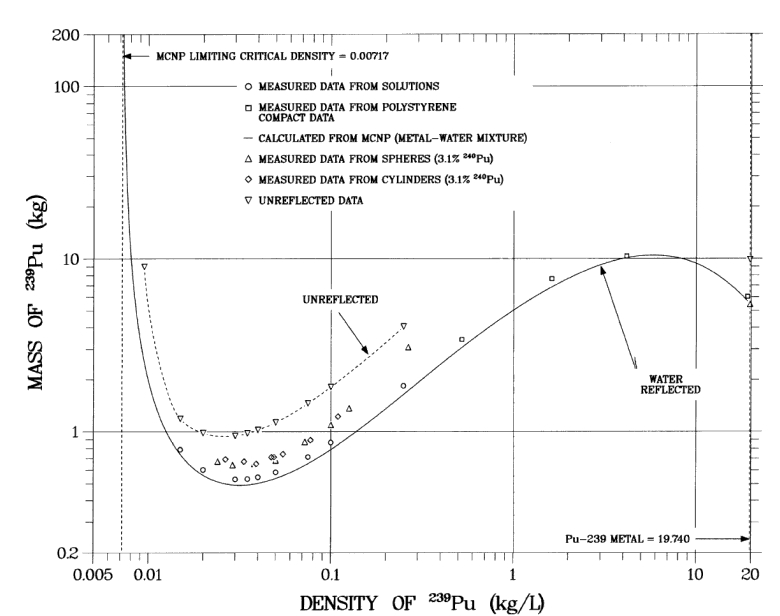
\includegraphics[keepaspectratio, width = 5.0 in]{images/pu_critical_mass}
    \caption{Pu-239 solution critical mass. (Borrowed from Martin, J. {
             Physics for Radiation Protection: A Handbook}, Wiley (2016).}
    \label{fig:pu_critical_mass}
\end{figure}

%------------------------------------------------------------------------------
% ACCIDENTS
%------------------------------------------------------------------------------

\section*{Accidents}

What exactly \textit{is} a criticality accident?  In the simplest terms,
it is an excursion, an uncontrolled chain reaction.  To help understand
accidents
both qualitatively and quantitatively, let's review a few ideas from
reactor kinetics.  Recall that \textit{reactivity} measures a departure
from criticality, and is most often expressed via
\begin{equation}
 \rho = \frac{k-1}{k} \, .
\end{equation}
Postive $\rho$ denotes a supercritical state, negative $\rho$ a 
subcritical state, and $\rho = 0$ is equivalent to $k=1$ or a 
critical state.  We can further differentiate between a \textit{delayed
critical} state and a \textit{prompt critical} state.  The latter 
occurs when $\rho > \beta$, where $\beta$ is the delayed neutron
fraction.  This situation is to be avoided in all but a few specific
experimental situations, for in the prompt critical regime, 
the growth of the neutron population occurs on timescales close
to the prompt neutron lifetime (say $10^{-8}$ to $10^{-4}$ seconds in many
systems of interest).  

To get an idea of the orders of magnitude we deal with in an accident
situation, consider a critical system with a constant neutron population
of just one neutron.  Suddenly, a perturbation brings the system
into a prompt critical state for a short time $\Delta t$.  During this
time, the population grows as $n \propto n_o e^{(\rho-\beta)t/\Lambda}$.  
Assuming $\Lambda = 10^{-5}$ seconds, $\rho-\beta = 0.002$, and the perturbation 
lasts two tenths of second\footnote{the average human reaction time is
about 200 milliseconds. 
See \url{http://www.humanbenchmark.com/tests/reactiontime/stats.php}}, 
we estimate that the number of neutrons produced is 
roughly
\begin{equation}
\begin{split}
 N &= \int^{0.5}_0 dt e^{(\rho-\beta)t/\Lambda} \\
   &= \frac{10^{-5}}{0.002} (e^{40} - 1) \\
   &\approx 1 \cdot 10^{15} \, .
\end{split}
\end{equation}
Suppose a worker is about a half a meter from the neutron source, so that
the fluence is $\Phi \approx 10^{15} / (4\cdot \pi \cdot 50^2)$ n/cm$^2$.
Looking up neutron fluence-to-dose equivalent factors (see 10CFR-20
\footnote{\url{http://www.nrc.gov/reading-rm/doc-collections/cfr/part020/part020-1004.html}}) 
suggests
that a high energy (1 MeV) fission fluence of $27\cdot 10^6$  n/cm$^2$
corresponds
to a dose of 1 rem.  Hence, our excursion yields a dose of around
1200 rem (12 Sv).  For perspective, a dose of 4 Sv is lethal roughly 
half the time.  Of course, this is a crude example, but it gives a 
very clear picture of the issues at hand.

In fact, the example above is not too far different than one of the first
documented criticality accidents from August of 1945.
Figure \ref{fig:pu_sphere} shows
a 6.2 kg plutonium sphere coated with nickel and surrounded by
blocks of tungsten carbide for reflection.  In the accident, an 
experimenter was placing blocks to achieve criticality.  While
placing the last block, the detector reading suggested that 
the block would actual produce a supercritical state.  Unfortunately,
the experimenter dropped the brick onto the assembly, yielding
a prompt supercritical excursion of $10^{16}$ fissions
before he was able to remove the brick.  A later study estimated
the resulting dose to be 510 rem, which proved to be fatal some
28 days later.  The same assembly would be involved in a second
fatal accident just months later, where the experimenter handled
one of two beryllium hemisphere reflectors
 with his thumb (in a hole in the 
hemisphere) and a screwdriver, a procedure Feynman dubbed
``tickling the dragon's tail.''   The screwdriver, holding the 
reflectors apart, slipped and caused an excursion that led to 
the experimenter's death 9 days later and significant doses
to observers; see Figure \ref{fig:pu_sphere_2} for a recreation
of the experiment.

\begin{figure}[ht] 
    \centering
    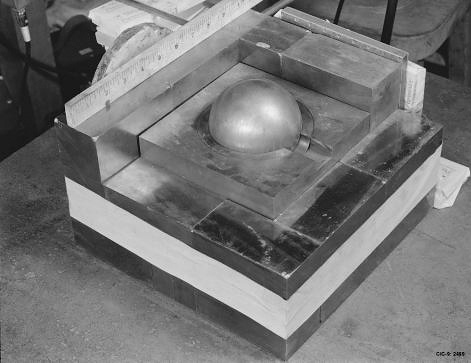
\includegraphics[keepaspectratio, width = 4.0 in]{images/pu_sphere}
    \caption{Plutonium sphere reflected by tungsten-carbide bricks.}
    \label{fig:pu_sphere}
\end{figure}

\begin{figure}[ht] 
    \centering
    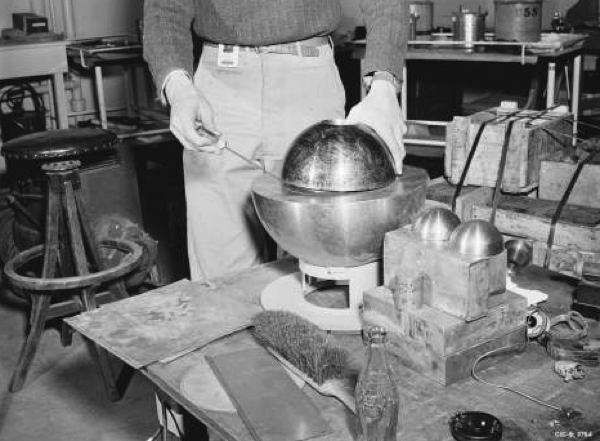
\includegraphics[keepaspectratio, width = 4.0 in]{images/pu_sphere_2}
    \caption{Recreation of the ``tickling the dragon's tail'' 
             experiment.}
    \label{fig:pu_sphere_2}
\end{figure}


A second type of accident involves processing operations in which
fissile materials are in solution.  The first domestic processing
accident occured at the Y-12 plant in Oak Ridge, TN.  Y-12 
produces parts from HEU for use in nuclear weapons.  

The accident occured in a portion of the plant used to 
recover HEU from waste material and place it in tanks of favorable
geometry.  These tanks were to be emptied, cleaned, and leak-tested 
with water.  Before the leak-testing began, however, uranium 
solution had leaked from the process stream into the piping
below the storage tanks (and actually into one of the tanks,
as its release valve had been let open).  When the other tanks, full
of water, were emptied, the uranium solution and water accumulated
in a 55 gallon drum.  A nearby worker first noticed dark yellow
fumes followed by a blue flash.  Eight workers received significant
doses, though none died as a result of acute effects.

Unfortunately, criticality accidents are not a thing of the past.  A 
recent example happened in Tokai-mura, Japan at a uranium conversion
plant.  The accident occurred when workers placed 16.6 kg of 18.8\%
enriched uranium into a tank designed to contain no more than
2.4 kg of uranium at such high enrichments.  The accident was the 
first of its kind in Japan, and the first resulting in casualties.
The accident is somewhat unique in that criticality was maintained
intermittently for roughly 20 hours before effective action was
taken.  

A rather complete history of criticality accidents in the U.S. and
around the world is contained in the latest edition of
 \textit{A Review of Criticality Accidents} from Los Alamos.  This
document is a really great piece of nuclear history, and students
are highly encouraged to skim through the many accidents covered.

%------------------------------------------------------------------------------
% Computational Aspects
%------------------------------------------------------------------------------

\section*{Computational Aspects}

The intent of this section to provide the reader with an 
overview of criticality safety analysis validation. A brief 
review of regulations and guidance pertinent to criticality safety of 
fissile materials outside reactors is given, with a particular emphasis on 
requirements for ensuring subcritical conditions. The traditional approach to 
bias determination is discussed, and one specific method used in practice
is described and demonstrated in an illustrative example. Subsequently, 
modern S/U-based validation techniques are discussed, and an 
illustrative example is provided and related to the traditional approach.

%------------------------------------------------------------------------------

\subsubsection{Subcritical Limits}

As noted above, ANSI/ANS-8.1 provides guidance 
for avoiding criticality accidents during handling of fissionable material 
outside of reactors \cite{ans8_1}. The standard provides basic safety principles 
in addition to several limits for simple systems of single isotopes.  
Specifically, the standard defines a \textit{subcritical limit} to be ``the 
limiting value assigned to a controlled parameter that results in a subcritical 
system under specified conditions. The parameter limit allows for 
uncertainties in the calculations and experimental data used in the derivation 
but not for contingencies.''

These limits are \textit{absolute maxima}, and since they do not include 
contingencies, in practice, adminstrative margins are employed.  A typical 
value, as we'll see below, tends to be 5\% on \keff.

Table \ref{tbl:controlparams} gives several examples of single control 
parameters used in criticality safety analysis.  Note, while ANSI/ANS 8.1 
specifies limits in terms of a single parameter, in some cases, multiple 
parameter limits are also employed.  The standard suggests a few examples, and
cites the technical literature for further guidance. However, while less 
conservative, multiple 
parameter limits require additional adminstrative margins and may be harder to 
use in validation.

\begin{table}[ht]
    \caption{Example single parameters and subcritical limits.}
    \begin{center} 
    \begin{tabular*}{0.90\textwidth}{@{\extracolsep{\fill}} ll } 
      \toprule 
	parameter &  example limit \\
      \midrule
       fissile mass                    &  0.78 kg ${}^{235}$U in UO$_2$NO$_3$ \\
       dimension (width, volume, etc.) &  6.2   L ${}^{235}$U in UO$_2$NO$_3$ \\
       concentration                   &  11.6 g/L${}^{235}$U in UO$_2$NO$_3$ \\
       enrichment                      &  5\%     ${}^{235}$U in UO$_2$       \\
       fissile mass                    &  20.1 kg ${}^{235}$U in UO$_2$ 
                                          (w/ $\rho \leq 18.81$ g/cc) \\
      \bottomrule 
    \end{tabular*} 
    \end{center} 
    \label{tbl:controlparams}
\end{table}

%------------------------------------------------------------------------------


\subsubsection*{Criticality Safety Analysis Validation}

While the single parameter limits provide useful guidance, two questions 
naturally arise.  First, how does one actually establish these limits?  And 
second, how does one ensure subcriticality in systems that are much more 
complex than, for example, a sphere?  The answer in both cases is by using 
computational methods validated against experiment.

In addition to the single parameter limits, ANSI/ANS-8.1 provides 
requirements for ensuring computational methods used in criticality safety 
analyses are both valid and within the ``area of applicability'' for specific 
applications. The standard defines the area of applicability as ``limiting 
ranges of material compositions, geometric arrangements, neutron energy 
spectra, and other relevant parameters \ldots within which the bias of the 
calculational method is established'' \cite{ans8_1}.  In other words, an 
\textit{application} is the system of interest, such as a spent fuel canister 
for shipment and disposal. A computational method is \textit{applicable} if 
it is verified against a set of \textit{experiments} that are similar to the 
application with respect to composition, geometry, and so forth.

A \textit{computational bias} is the systematic 
discrepancy between and experimental data and calculated results. Biases 
have associated uncertainties, which quantify the accuracy and 
precision of calculated values and the uncertainty in measured data.

When computational tools are used in criticality safety analyses, the standard
requires that the bias be established.  Qualitatively, the bias must be 
determined via correlating data from critical experiments to computational 
models of the same experiments using the tool to be validated. 
Typically, the measured and 
computed values of \keff are related, but other physical quantities may 
also be used.  The bias is used to normalize a particular code within its 
area of applicability so that its results, after applying the bias, may be 
used to predict criticality within the bias uncertainty.

Another American National Standard, ANSI/ANS-8-17, further explicates 
use of computational tools by defining specific criteria for establishing 
subcriticality \cite{ans8_17}.  Whenever computational methods are 
used in criticality safety analyses, the standard requires that the calculated 
application multiplication factor $k_a$ must be less than or equal to the 
allowable multiplication factor.

The easiest way to think of this is to note that the largest, ``worst case'' 
value for $k_a$ must be below the smallest, least conservative computed 
estimate.  That is to say, the maximum expected application multiplication 
factor (\ie $k_a + \Delta k_a$) must be less than the minimum expected 
computed value (\ie $k_c - \Delta k_c$) for an applicable critical experiment, 
\ie a real, measured system whose \keff is unity, or an average computed 
\keff for several such experiments.  Mathematically, this can be written as
\begin{equation}
 k_a + \Delta k_a \leq k_c - \Delta k_c \, ,
\end{equation}
or
\begin{equation}
 k_a \leq k_c  - \Delta k_a - \Delta k_c \, .
\end{equation}
For added conservatism, the standard further requires that
\begin{equation}
 k_a \leq k_c - \Delta k_a - \Delta k_c - \Delta k_m \, ,
\label{eq:kapp}
\end{equation}
where the standard defines:

\begin{tabular}{rp{10cm}}
 $k_a$           & is the calculated \keff of the 
                   application system for all normal or credible 
                   abnormal conditions; \\
\end{tabular}

\begin{tabular}{rp{10cm}}
 $k_c$           & is the average \keff from the calculation of 
                   the benchmark criticality experiments. 
                   The experiments used 
                   should be neutronically similar to the application
                   system. If the application system has 
                   parameters beyond the area of applicability established 
                   by the benchmark experiments, then the area of 
                   applicability
                   may be extended using trends in the calculated values 
                   of $k_c$ as functions of those parameters; \vspace{12pt} \\
\end{tabular}

\begin{tabular}{rp{10cm}}
 $\Delta k_a$    & is an allowance for 
                 \begin{itemize}
                   \item statistical or convergence uncertainties in 
                         the computed $k_a$;
                   \item material and fabrication tolerances;
                   \item uncertainties due to geometry or material
                         simplifications and approximations;
                 \end{itemize}  \\
\end{tabular}

\begin{tabular}{rp{10cm}}
 $\Delta k_c$    & is a margin for uncertainty in $k_c$ that includes 
                   allowances for
                 \begin{itemize}
                   \item uncertainties in the critical experiments;
                   \item statistical or convergence uncertainties
                         in the computated $k_c$;
                   \item uncertainties due to extrapolation of $k_c$ 
                         outside the experimental data range;
                   \item uncertainties due to geometry or material
                         simplifications and approximations;
                 \end{itemize}
\end{tabular}

\begin{tabular}{rp{12cm}}
 $\Delta k_m$    & is an arbitrary ``administrative'' 
                   margin to ensure the subcriticality 
                   of $k_a$. \\
\end{tabular}

Eq. \ref{eq:kapp} can be rewritten as
\begin{equation}
 k_a + \Delta k_a + \Delta k_m - \beta + \Delta \beta \leq 1 \, ,
\label{eq:kallow}
\end{equation}
where $\beta = k_c - 1$ is the bias and $\Delta \beta = \Delta k_c$ is the 
uncertainty in the bias.  The definition of $\beta$ is based on the fact 
that critical experiments, by their definition, have \keff = 1, and hence 
the bias is just the difference between the computed value and unity.  By 
convention, the bias is defined such that a \textit{ negative} $\beta$ 
indicates an \textit{ underestimated} \keff\!, which is undesirable.

To ensure subcriticality in the application system, an \textit{ upper 
subcritical limit} is defined as
\begin{equation}
 USL = 1 - \Delta k_m + \beta - \Delta \beta \, ,
\label{eq:usl}
\end{equation}
and from Eq. \ref{eq:kallow}, it is apparent that $k_a + \Delta k_a \leq USL$ 
\cite{lichtenwalter1997cbg}.   Thus, the USL is the maximum value an 
application \keff (plus any uncertainties) may have for which the 
application can, with a high degree of confidence, be considered 
subcritical.  The value $1 - USL$  is the mathematical definition of the 
subcritical margin.  In the event the bias $\beta$ is positive, \ie the 
computed value $k_c$ overestimates \keff\!, current practice is to set 
the bias to zero rather than reduce the subcritical margin.

%------------------------------------------------------------------------------

\subsubsection{Traditional Bias Determination}

In the United States, biases and associated uncertainties and USL's have 
often been found through use of \textit{ trending analysis}.  A suite of 
critical experiments is selected for use in a specific safety analysis 
based on the similarity of the experiments to the safety analysis system.  
Traditionally, this similarity is based on physical parameters that include 
the fissile material, hydrogen-to-fissile atom ratio (H/X), average neutron 
energy group causing fission, and energy of average lethargy causing 
fission (EALF), among others \cite{broadhead2004sau}.

While various methods using trending analysis exist for determining the 
biases and USL's, one common approach, denoted USL$_1$ in the 
literature \cite{broadhead2004sau}, is discussed here to provide at least 
some background of current practice. The following description is largely 
adapted from the technical report in which it was first developed 
\cite{lichtenwalter1997cbg}. 

The method computes $k_c(x)$ as a function of a trending parameter $x$ 
using linear regression.  The bias, $\beta(x)$, is just $k_c(x) - 1$.  .  

A lower confidence band $w(x)$ is statistically computed using current 
experiments and uncertainties as well as a specified confidence.  This 
confidence band defines the value below which an additional computed 
\keff value (\ie not included in the analysis) must be for the additional 
system to be considered subcritical with a high degree of confidence.  
Equivalently, for a given value of the trending parameter $x$, $w(x)$ 
represents the value \textit{ above} which the additional computed value $k_c$ 
will be \textit{ if} the system in question is critical---and this consequently 
implies any negative $\beta(x)$ is no worse than $w(x) - 1$.  Hence, if our 
aim is to ensure the actual \keff of a system is subcritical, then its 
computed value should be \textit{ less} than the appropriate confidence band 
value.

To simplify analyses, the limiting width, $W$, of the confidence band is 
used, which (like $w(x)$) takes into account all uncertainties associated 
with the experiments (\eg experimental, stochastic, etc), and consequently, 
is a statistical measure of $\Delta \beta$.  The width $W$ of the 
confidence band is defined
\begin{equation}
 W = \mathrm{max} \Big \{ w(x) | x_{\mathrm{min}},x_{\mathrm{max}} \Big \} \, ,
\label{eq:confwidth}
\end{equation}
where
\begin{equation}
 w(x) = t_{1-\gamma} s_p \Bigg ( 1 + \frac{1}{n} + 
        \frac{(x-\bar{x})^2}{\sum^n_{i=1} (x_i - \bar{x})^2} \Bigg )^{1/2} \, ,
\end{equation}
and $n$ is the number of critical experiments included in the analysis, 
$t_{1-\gamma}$ is the student-t distribution statistic for $1-\gamma$ 
and $n-2$ degrees of freedom ($\gamma$ is the desired confidence level), 
$\bar{x}$ is the mean value of $x$ in the set of experiments, and $s_p$ 
is the pooled standard deviation for the set of calculations.

The pooled standard deviation $s_p$ is defined by
\begin{equation}
 s^2_p = s^2_{k(x)} + s^2_w \, ,
\end{equation}
where $s^2_{k(x)}$ is the mean-square error of the linear regression, 
defined as
\begin{equation}
 s^2_{k(x)} = \frac{1}{n-2} \Bigg ( \sum^n_{i=1} (k_i - \bar{k})^2 - 
              \frac{\Big(\sum^n_{i=1} (x_i-\bar{x})(k_i -\bar{k}) \Big )^2 }
                   {\sum^n_{i=1} (x_i - \bar{x})^2} \Bigg ) \, ,
\end{equation}
and $s^2_w$ is the variance of the data, defined as
\begin{equation}
 s^2_w = \frac{1}{n} \sum^n_{i=1} \sigma^2_i \, ,
\end{equation}
where  $\sigma_i$ is the uncertainty in the $i$th calculated value, 
accounting for method uncertainty (\eg Monte Carlo statistics) and 
estimated uncertainty due to cross-section uncertainty.

The width of the confidence $W$ is chosen to be the \textit{ maximum} value 
of $w$ at the limits of the range of $x$ corresponding to the experiments 
to be conservative, and moreover, it serves to simplify the definition of 
USL.  Current guidance is to define $W$ at the 95\% confidence level, 
\ie choose $\gamma = 0.95$.  Below, we provide an
illustrative example of the USL$_1$ methodology.

%------------------------------------------------------------------------------

\subsubsection{S/U-Techniques}

Unfortunately, the proper selection of parameters over which to trend, 
and the experiments with which to trend, is largely based on expert 
judgement.  As experiments continue to become more expensive, use of 
computational methods will grow.  Furthermore, new applications will 
continue to extend beyond the areas of applicability of current 
experimental data, and consequently, methods to extend beyond these 
areas are needed.

For the past several years, ORNL has worked with the support of the 
NRC and the Department of Energy's (DOE) Nuclear Criticality Safety 
Program to develop ``a rigorous physics-based approach for the 
determination of system similarity'' for determining areas of 
applicability \cite{broadhead2004sau}.  Additionally, their efforts 
aimed to develop the methodology and computational tools needed for 
``determination of biases and uncertainties due to experimental 
descriptions, computational methods, and nuclear data.''

As an alternative to traditional trending analysis, work was done to 
develop S/U-based, easily-quantifiable parameters to measure the 
similarity of systems.  It is beyond our scope to describe the 
methods in detail.  Interested readers should see the exercises
of Lecture \ref{lec:the_adjoint_and_perturbation_theory} for some
basic theory needed to derive the results, and Ref. 
\cite{broadhead2004sau} for greater detail.

Skipping the theory, what we end up with is the sensitivity
of \keff to the various underlying nuclear data, 
\begin{equation}
 S_{k,\sigma_x} = \frac{\sigma_x}{k}\frac{\partial k}{\partial \sigma_x} 
 \label{eq:keffsens}
\end{equation}
where $x$ denotes some reaction of interest.  We express the sensitivity 
of \keff to all nuclides in a system as the vector $\mathbf{S}_k$,
which can implicitly represent dependence on multigroup data.

Sensitivity vectors can be used to compare both the qualitative and 
quantitative similarity between two systems with respect to single or 
several nuclide-reactions. Let the entire set of group-wise, nuclide-reaction 
cross-sections be denoted 
$\bm{\sigma} \equiv \sigma_i, \; \; n = 1,\;2,\ldots,N$, where $N$ is the 
total number of nuclide-reactions multiplied by the number of energy 
groups.  The $N\times N$ correlation (\ie relative covariance) matrix 
of $\bm{\sigma}$ is defined
\begin{equation}
\mathbf{C_{\sigma \sigma}} \equiv \Bigg[\frac{\mathrm{COV}(\sigma_i,\sigma_j)}
                                             {\sigma_i \sigma_j} \Bigg ] \, ,
\end{equation}
where $i$ and $j$ range from 1 to $N$, and 
\begin{equation}
\mathrm{COV} = \langle (\sigma_i - \bar{\sigma_i})(\sigma_j - 
               \bar{\sigma_j}) \rangle 
             = \langle \delta \sigma_i \delta \sigma_j \rangle \, ,
\end{equation}
where $\bar{\sigma_i}$ represents the expected value of the data $\sigma_i$.  

Because the components of \cov represent relative uncertainties, and because 
from above, we know the \keff sensitivity represents the relative change in 
\keff due to relative changes in some nuclide-reaction data, the relative 
uncertainty in \keff is therefore
\begin{equation}
\frac{\delta k}{k} = \sqrt{ \mathbf{S}_k \mathbf{C_{\sigma \sigma}} 
                     \mathbf{S}_k^T } \, ,
\end{equation}
where $T$ denotes the matrix transpose.  If several systems are of interest, 
then an $N \times I$  matrix of sensitivity vectors $\mathbf{\bar{S}}_k$ can 
be defined, where $I$ is the number of systems.  By folding 
$\mathbf{\bar{S}}_k$ with \cov, one obtains
\begin{equation}
 \mathbf{C}_{kk} =  \mathbf{\bar{S}}_k \mathbf{C_{\sigma \sigma}} 
                    \mathbf{\bar{S}}_k^T  \, ,
\label{eq:kunc}
\end{equation}
an $I\times I$ matrix consisting of each system's relative variance in 
\keff (\ie $(\Delta k/k)^2$) due to data uncertainties (the diagonal terms, 
$\alpha_{ii}$) and the relative covariances in \keff between systems 
(the off-diagonal terms, $\alpha_{ij}$).  These off-diagonal terms 
represent ``shared variance'' or ``shared uncertainty'' between systems.  

The correlation coefficient between system $i$ and $j$ is defined
\begin{equation}
 c_{k} =  \frac{\alpha^2_{ij}}{\alpha_i \alpha_j}  \, ,
\label{eq:ck}
\end{equation}
which, as is expected, takes on values between -1 
(completely anti-correlated) and 1 (completely correlated). 
A value $c_k = 0$ indicates no correlation between systems.  

The correlation of two systems is greatest if they share basic 
characteristics, \eg fuel type, moderator, other materials.  Two 
water-moderated thermal UO$_2$ systems would be expected to have 
a higher degree of correlation than would such a thermal system 
and a molten salt fast reactor.  Use of $c_k$ as a trending 
parameter in the USL$_1$ method is illustrated below.

%------------------------------------------------------------------------------

\subsubsection{Example Analyses}

To illustrate the USL$_1$ method using both traditional parameters 
and $c_k$, 25 thermal LEU systems were chosen for example analyses.  
Two additional systems were selected as ``applications'' for which 
the $\beta$, $\Delta \beta$, and the USL are determined\footnote{The 
minimum recommended number of experiments for trending with the 
USL$_1$ method is 25; here, just the minimum was used for these example 
cases.}. The experiments range from 2.35\% to 5\% enrichement, and have 
EALF values ranging from 0.017 to 2.24 eV.  %These parameters, along 
%with $c_k$ with respect to the two applications (LCT-079-002 and 
%LCT-050-001), are provided in Table \ref{tbl:exampletrend}. 
All experiments 
are included in the International Handbook of Evaluated Criticality Benchmark 
Experiments \cite{ihecsbe} and are low enriched uranium, thermal assemblies.
The LCT-079 and LCT-050 are experiments
of use to burnup credit, a topic discussed below; however, their use here
is purely for example.  

Figures \ref{fig:trend_ealf}-\ref{fig:trend_ck2} show the trending analysis 
for using EALF, enrichment, and $c_k$.  For both EALF and enrichment, only 
one analysis was needed for the applications since neither parameter depends 
on the application.  However, separate cases were run using $c_k$ values 
specific to the given application.  The experiments are the black dots, 
and the applications are red shapes.  For all cases, the uncertainty is 
computed using Eq. \ref{eq:kunc}, where the uncertainty for the system is 
its associated diagonal element of $\mathbf{C}_{kk}$, \ie the uncertainty 
in cross-sections propagated to \keff via use of sensitivity profiles.  
This is in line with previous analyses \cite{broadhead2004sau}.  Note, for 
the USL, an administrative margin of $\Delta k_m = 0.05$ was used.

% \begin{table}[hp]
%  \caption{Experiment and test application parameters.  Note (a) and (b) refer to the LCT-079 and LCT-050 experiments.}
%  \begin{center} 
%  \begin{tabular*}{0.95\textwidth}{@{\extracolsep{\fill}} ccccccc } 
%   \toprule 
%          Id.       &  \keff   & $\sigma_k$&  EALF (eV)&  Enrich.(\%) & $c_k$ (a) & $c_k$ (b)    \\ 
%    \midrule
%   LCT-010-005  &  0.9951  &  0.0050  &  3.89E-01  &  4.306  &  0.861  &  0.890  \\
%   LCT-010-016  &  0.9936  &  0.0058  &  2.92E-01  &  4.306  &  0.977  &  0.982  \\
%   LCT-010-017  &  0.9937  &  0.0058  &  2.86E-01  &  4.306  &  0.979  &  0.983  \\
%   LCT-010-018  &  0.9924  &  0.0058  &  2.81E-01  &  4.306  &  0.980  &  0.985  \\
%   LCT-010-019  &  0.9917  &  0.0058  &  2.74E-01  &  4.306  &  0.980  &  0.986  \\
%   LCT-017-003  &  0.9927  &  0.0055  &  9.57E-02  &  2.350  &  0.899  &  0.924  \\
%   LCT-017-004  &  0.9919  &  0.0052  &  2.17E-01  &  2.350  &  0.827  &  0.850  \\
%   LCT-017-005  &  0.9945  &  0.0053  &  1.89E-01  &  2.350  &  0.851  &  0.876  \\
%   LCT-017-006  &  0.9939  &  0.0054  &  1.78E-01  &  2.350  &  0.862  &  0.888  \\
%   LCT-017-007  &  0.9937  &  0.0053  &  1.69E-01  &  2.350  &  0.858  &  0.884  \\
%   LCT-042-001  &  0.9906  &  0.0054  &  1.73E-01  &  2.350  &  0.797  &  0.764  \\
%   LCT-042-002  &  0.9909  &  0.0055  &  1.79E-01  &  2.350  &  0.801  &  0.767  \\
%   LCT-042-003  &  0.9897  &  0.0054  &  1.86E-01  &  2.350  &  0.779  &  0.747  \\
%   LCT-042-004  &  0.9918  &  0.0054  &  1.84E-01  &  2.350  &  0.768  &  0.736  \\
%   LCT-042-005  &  0.9921  &  0.0057  &  1.81E-01  &  2.350  &  0.891  &  0.862  \\
%   LCT-049-001  &  0.9904  &  0.0057  &  2.02E+00  &  5.000  &  0.889  &  0.860  \\
%   LCT-049-002  &  0.9914  &  0.0057  &  2.03E+00  &  5.000  &  0.895  &  0.867  \\
%   LCT-049-003  &  0.9913  &  0.0055  &  2.15E+00  &  5.000  &  0.877  &  0.849  \\
%   LCT-049-004  &  0.9906  &  0.0058  &  2.24E+00  &  5.000  &  0.932  &  0.910  \\
%   LCT-049-005  &  0.9915  &  0.0059  &  1.14E+00  &  5.000  &  0.934  &  0.911  \\
%   LCT-049-006  &  0.9900  &  0.0055  &  1.15E+00  &  5.000  &  0.889  &  0.894  \\
%   LCT-049-007  &  0.9904  &  0.0053  &  1.11E+00  &  5.000  &  0.873  &  0.878  \\
%   LCT-049-008  &  0.9906  &  0.0053  &  1.19E+00  &  5.000  &  0.862  &  0.867  \\
%   LCT-049-009  &  0.9912  &  0.0053  &  7.39E-01  &  5.000  &  0.869  &  0.873  \\
%   LCT-049-010  &  0.9904  &  0.0053  &  7.47E-01  &  5.000  &  0.869  &  0.874  \\
%   \midrule
%   LCT-079-002  &  0.9897  &  0.0069  &  2.03E+00  &  4.310  &  1.000  &  na     \\
%   LCT-050-001  &  0.9906  &  0.0067  &  1.99E-01  &  4.738  &  na     &  1.000  \\
%   \bottomrule 
%  \end{tabular*} 
%  \end{center} 
%  \label{tbl:exampletrend}  
% \end{table}

\begin{figure}[htp] 
    \centering
    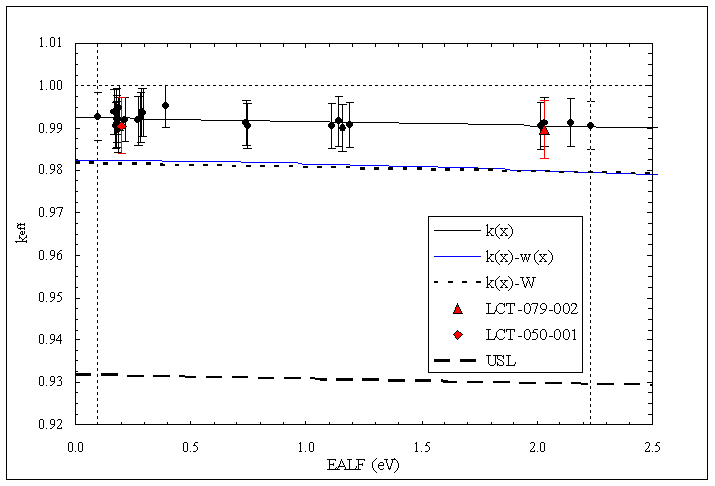
\includegraphics[keepaspectratio, width = 5 in]{images/trend_ealf}
    \caption{Example trending analysis using EALF.}
    \label{fig:trend_ealf}
\end{figure}


\begin{figure}[htp] 
    \centering
    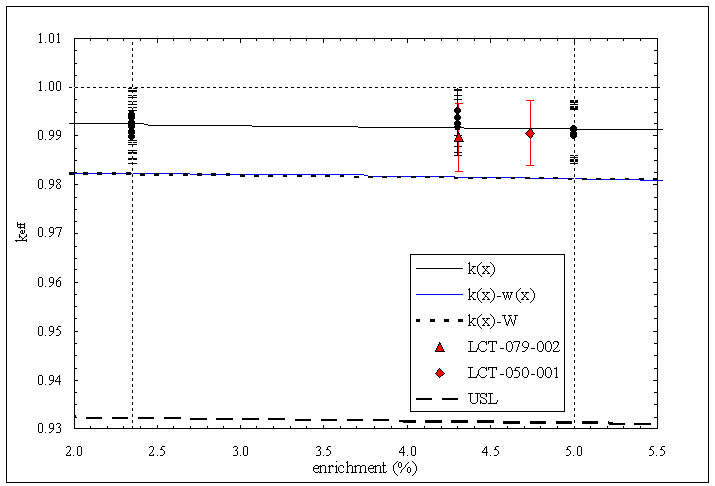
\includegraphics[keepaspectratio, width = 5 in]{images/trend_enrich}
    \caption{Example trending analysis using enrichment.}
    \label{fig:trend_enrich}
\end{figure}


\begin{figure}[htp] 
    \centering
    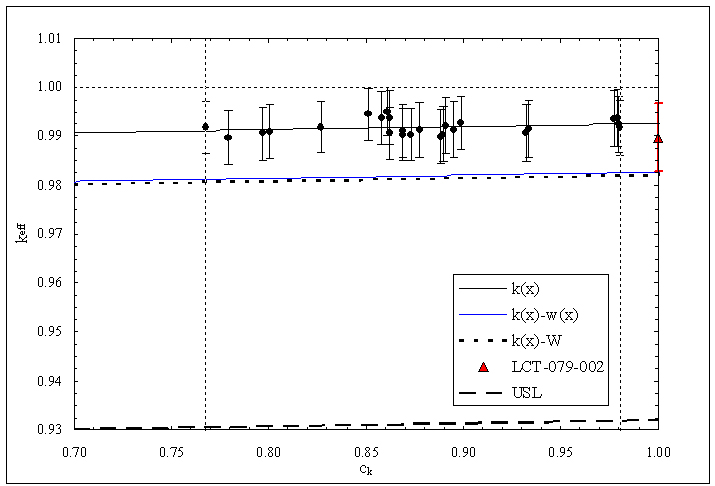
\includegraphics[keepaspectratio, width = 5 in]{images/trend_ck1}
    \caption{Example trending analysis using $c_k$ (for LCT-079-002).}
    \label{fig:trend_ck1}
\end{figure}


\begin{figure}[htp] 
    \centering
    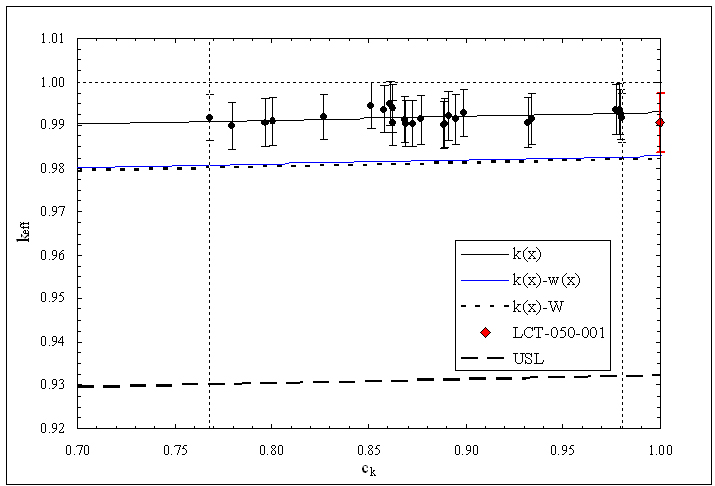
\includegraphics[keepaspectratio, width = 5 in]{images/trend_ck2}
    \caption{Example trending analysis using $c_k$ (for LCT-050-001).}
    \label{fig:trend_ck2}
\end{figure}

From the trends, the bias $k(x)-1$ (where $x$ is the parameter value 
for the application) and associated bias uncertainty (\ie $W$ from 
Eq. \ref{eq:confwidth}) can be computed in addition to the USL.  
Since the ``applications'' are known critical experiments, it is useful 
to compare the observed bias (\ie $k_{\mathrm{calc}} -1$) to the bias 
as predicted via trending.  Table \ref{tbl:trendbias} provides the 
observed and predicted biases (with uncertainty) and the USL for both 
applications.  For each application, all three methods yield very similar 
USL's, and all the biases are slightly underpredicted but well within 
one standard deviation of the observed biases.  

With such a large $\Delta k_m$, it is easy to wonder why we care 
about $\Delta \beta$. However, if we interpret subtracting $\Delta k_m$ 
from \keff as simply shifting the definition of critical, then it 
becomes clearer that $\Delta \beta$ is still important.

{\tiny
\begin{table}[hp]
 \caption{Observed and predicted biases ($\beta_{\mathrm{ob}}$ and 
         $\beta$), $\Delta \beta$, all in percent, and USL using 
         each trending technique.}
 \begin{center} 
 \begin{tabular*}{0.98\textwidth}{@{\extracolsep{\fill}} c|cccc|cccc } 
  \toprule
              & \multicolumn{4}{c}{LCT-079-002}          & \multicolumn{4}{c}{LCT-050-001} \\
   \midrule 
             & $\beta_{\mathrm{ob}}$ & $\beta$ & $\Delta \beta$  & USL & $\beta_{\mathrm{ob}}$& $\beta$  & $\Delta \beta$ & USL \\ 
   \midrule
       EALF  &  -1.08  &  -0.95  &  1.08  &  0.9298  &  -0.94  &  -0.77  &  1.08  &  0.9316 \\
    Enrich.  &  -1.08  &  -0.84  &  1.02  &  0.9314  &  -0.94  &  -0.85  &  1.02  &  0.9313 \\
      $c_k$  &  -1.08  &  -0.74  &  1.16  &  0.9306  &  -0.94  &  -0.71  &  1.07  &  0.9322 \\
  \bottomrule 
 \end{tabular*} 
 \end{center} 
 \label{tbl:trendbias}  
\end{table} 
}

\section*{Case Study: Burnup Credit}

\subsubsection*{Overview and Motivation}

The transportation and storage of used nuclear fuel is an integral component of any
nuclear fuel cycle. During handling of used nuclear fuel, strict attention must be paid
to criticality safety. The chief concern of criticality safety is to ensure the effective
multiplication factor \keff of the system in question is below unity at all times, i.e. to
ensure subcriticality.
For the case of used nuclear fuel, several factors affect the subcritical margin, i.e.
by how much a system is subcritical. Typical, unirradiated light water reactor (LWR)
fuel consists of uranium-oxide (UO2 ) enriched to 3-5\% ${}^{235}$U. During its time in the
reactor, nuclear fuel undergoes significant compositional changes, a process referred
to as burnup. Most importantly, the fissile isotope 235 U is depleted, generating various
fission products (FP's), many of which are parasitic neutron absorbers. Simultaneously,
${}^{235}$U breeds ${}^{239}$Pu which also undergoes fission and produces FP's. The net
effect of these compositional changes is to decrease the \keff of the fuel with increased
burnup. Accounting for this decrease in \keff (or equivalently, a decrease in reactivity)
in subcritical margins is often referred to as \textit{burnup credit}.

Historically, the so-called \textit{fresh fuel assumption} was used as a conservative bound
in criticality safety analysis of used nuclear fuel [1]. More recently, the Nuclear
Regulatory Commission (NRC) offered guidance for crediting the major (fissile) actinides
in such analyses in its Interim Staff Guidance - 8, revision 2 (ISG-8R2) report [2]. However,
even this results in a very conservative estimate of the subcritical margin of used
nuclear fuel.

Changes in the major actinides account for about 66-75\% of the net reduction
in reactivity; FP's account for the remainder, the percentages depending on burnup.
The FP's relevant to burnup credit, roughly in order of importance, include SM.
 
Why do we care?  Naturally, assuming a canister of some number of burned assemblies 
contains only fresh fuel is quite conservative.  Figure \ref{fig:loading_curve} shows 
loading curves for a generic used fuel canister with 32 WH 17x17 assemblies of varying 
initial enrichments and burnups.  Configurations below a given line do not meet subcritical 
limits under the given assumptions.  The reference case assumes fresh fuel, and each 
subsequence curve relaxes the assumptions.  

Considering that much of the current U.S. inventory of used fuel lies below the reference 
curve, a 32-assembly canister could not be widely used (and instead, canisters such as
the 21-assembly Transportation, Aging, and Disposal (TAD) canister \cite{tad} 
intended for ultimate
disposition in Yucca Mountain would be required).  The cost of producing, loading, shipping, 
and disposing canisters is not negligible, and a study by Parks and Wagner suggest that
crediting the FP's in criticality safety analysis, thus allowing the high capacity
canisters, would potentially save upwards of \$200 million dollars in total disposal
costs \cite{parks2004csp}. 

\begin{figure}[ht] 
    \centering
    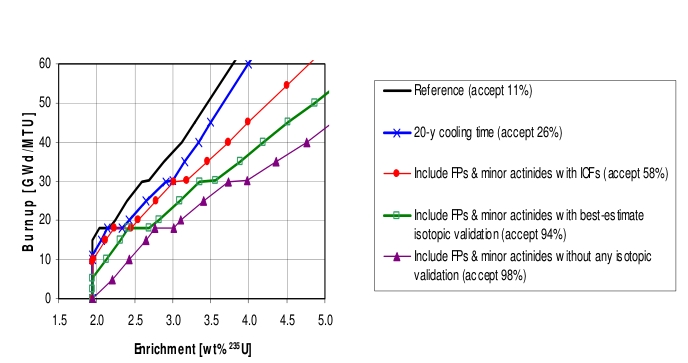
\includegraphics[keepaspectratio, width = 5.0 in]{images/loading_curve}
    \caption{Effect of calculational assumptions on loading curves for the GBC-32 and WH 17x17 assemblies.}
    \label{fig:loading_curve}
\end{figure}

\subsubsection*{Current Research}

To take into account the reduction in reactivity due to fission products,
called \textit{full burnup credit}, requires adequate knowledge of the 
isotopic content of the spent fuel (via validated depletion methods), and, 
our focus here, \textit{methods} to determine criticality and 
\textit{experiments} to validate those methods.

Current work has expanded on the S/U-based techniques
outlined above to develop methods for determinining biases of 
individual nuclides. While the details are beyond our scope, we give 
a brief description and several references for interested readers.

The basis of the work is the generalized linear least-square method (GLLSM).
GLLSM takes as input a set of nuclear data and covariances, the sensitivities 
of experiment models to nuclear data, the model \keff and uncertainty,
the experiment \keff and uncertainty (and any experiment correlation), 
and \textit{adjusts the nuclear data}
so that the the experiment and model \keff match.  It does so in a way that
minimizes the variation of all parameters (data and \keff) in terms of the
standard deviations of those parameters.  In other words, for all parameters
$p$, the method forces the experiment and model \keff to match while 
minimizing $\sum_i (\Delta p_i / \sigma_{p_i})^2$.  The adjustments can be 
propogated to an application's \keff via its model sensitivities, and the 
resulting difference is the bias.

To find biases of individual nuclides, the GLLSM method can be applied to 
so-called ``replacement experiments''.  These experiments consists of a single
reference case, and one or more cases that introduce some small perturbation
to the system, such as small foils of a fission product between fuel pellets 
 or small concentrations of a fission product in a bulk
moderator.  GLLSM can then be applied to the reactivity 
difference between a reference-perturbation pair of models and experiements 
(rather than on the eigenvalue), since the sensitivities of the 
reactivity difference should be small for all but the perturbation 
material.  Consequently, the corresponding adjustment to the data should 
primarily be due to the test material, and as above, the adjustment can 
be propagated to the application to define a nuclide-specific bias.

\subsubsection{Limitations}

Two significant limitations apply to the methods under development.  First,
the methods require that relevant experiments are available.  However,
only a handful of experiments have been performed relevant to burnup credit,
and of those, the difference between reference and perturbation cases may 
be too high to extract partial biases.  Moreover, little data is available
for the correlation between experiments.  For the the reactivity difference
method described above, the resulting biases are extremely sensitive to 
the correlation between experiments. This suggests that future 
experiments should be designed with the various S/U methods as guidance.

A second, perhaps more significant issue is the general lack of reliable
nuclear covariance data.  Only for the most important isotopes does credible
data exist (such as uranium isotopes).  For isotopes of generally less
importance (like many fission products), little if any covariance data
exists.  Until reliable covariance data exists, the methods described
above are of limited value.
 
\section{Further Reading}

Much of the content in this lecture was inspired by Knief's 
\textit{Nuclear Criticality Safety: Theory and Practice} \cite{knief1991ncs}. 
 Of
course, in one lecture, all that material cannot be covered, and the student
is directed to that book for more info most of the topics addressed here.
A more succinct overview of some of the topics is given by 
Pevey in a chapter of the \textit{Nuclear Engineering Handbook} 
\cite{pevey2010neu}.  

For an overview of the application of sensitivity and uncertainty analysis
to criticality safety, see Broadhead et. al \cite{broadhead2004sau}, and
for the latest work on adjustment techniques applicable to full burnup
credit, see Rearden et al. \cite{rearden2011sua}.